%% cap03-shorter-hesus-speaks.tex — Metodología

\chapter{Metodología}
\label{cap:metodologia}

\begin{quote}\small\textit{
Nota al lector: En este capítulo busqué explicar la metodología de forma accesible para lectores sin formación en programación o procesamiento de lenguaje natural. Cada herramienta se describe por lo que hace, no por cómo se programa. Lo relevante es entender la lógica del diseño: por qué primero se descubren temas sin categorías previas, luego se miden dimensiones específicas, y al final se verifica que el idioma no distorsione los resultados.
}\end{quote}


\section{Diseño de la Investigación}

El estudio es exploratorio, documental y comparativo~\citep{hernandez2014metodologia}. Es exploratorio porque no parte de una hipótesis que confirmar, sino de preguntas abiertas sobre qué temas caracterizan las políticas y en qué convergen~\citep{bowen2009document}. Es documental porque la fuente de datos son textos oficiales publicados por gobiernos. Es comparativo porque el análisis se estructura como una comparación entre países, en la tradición de la educación comparada.

El apoyo computacional no convierte al estudio en cuantitativo. Las herramientas de procesamiento de lenguaje natural funcionan como amplificadores de la capacidad analítica del investigador, no como sustitutos de su juicio~\citep{grimmer2013text}. Las herramientas detectan proximidad entre fragmentos de texto. La interpretación de qué significa esa proximidad en términos de política educativa corresponde al investigador.

\citet{nelson2020computational} propuso una secuencia para combinar análisis computacional con investigación cualitativa: primero se descubren patrones sin imponer categorías, luego se refinan con la lectura del investigador y después se confirman computacionalmente. Esta investigación sigue esa secuencia, adaptada al contexto de la educación comparada.


\section{Corpus Documental}

El corpus se compone de 13 documentos de política de siete países, seleccionados para representar regiones, idiomas y niveles de desarrollo distintos. Seis países contribuyen un documento principal cada uno. China contribuye siete documentos publicados entre 2017 y 2025, lo que permite observar cómo evolucionó su política a lo largo de ocho años. La Tabla~\ref{tab:corpus-shorter} presenta el corpus completo.

\begin{table}[htbp]
\centering
\caption{Corpus documental}
\label{tab:corpus-shorter}
\small
\begin{tabular}{lllll}
\hline
\textbf{País} & \textbf{Región} & \textbf{Documento} & \textbf{Año} & \textbf{Idioma} \\
\hline
EE.UU. & Norteamérica & Executive Order 14110 & 2023 & EN \\
Canadá & Norteamérica & Pan-Canadian AI Strategy & 2017 & EN \\
Colombia & Latinoamérica & CONPES 3975 & 2019 & ES \\
Alemania & Europa & KI-Strategie (actualización) & 2020 & DE \\
Sudáfrica & África & PC4IR Report & 2020 & EN \\
Australia & Oceanía & AI Action Plan & 2021 & EN \\
China & Asia & 7 documentos (2017--2025) & 2017--2025 & ZH$\rightarrow$EN \\
\hline
\end{tabular}
\end{table}

Los criterios de selección fueron cuatro: que el país contara con un documento oficial de IA que incluyera educación, que el conjunto representara diversidad geográfica y lingüística, que los documentos fueran de acceso público, y que hubieran sido publicados entre 2017 y 2025.

Los documentos de China se analizan en traducción al inglés realizada mediante el modelo Qwen 2.5, con revisión manual posterior del investigador. Los documentos de Alemania se analizan en su versión oficial en alemán. El corpus abarca cuatro familias lingüísticas (inglés, español, alemán y chino), lo que permite observar si el idioma de los documentos influye en las similitudes que el análisis detecta.


\section{Cómo se Analizan los Textos}

El análisis computacional de textos de política pública se ha consolidado en la última década como un campo con herramientas validadas para la investigación social~\citep{grimmer2013text}. Esta sección explica las tres herramientas que se utilizan, sin asumir conocimientos previos de programación.

\subsection{Representación semántica}

La técnica central consiste en convertir cada fragmento de texto en una coordenada dentro de un espacio conceptual. Textos que hablan de temas parecidos quedan cerca en ese espacio, aunque estén escritos en idiomas diferentes. Esta conversión la realiza un modelo de lenguaje entrenado en millones de textos en más de 50 idiomas~\citep{reimers2019sentencebert}.

Para hacer esto posible, cada documento se divide primero en fragmentos de aproximadamente un párrafo (800 caracteres con 200 de solapamiento entre fragmentos consecutivos). Cada fragmento se convierte en una lista de 384 números que representan su significado. Dos fragmentos que tratan el mismo tema producen listas numéricas parecidas, lo que permite medir cuánto se parecen mediante una fórmula estándar llamada similitud del coseno.

El modelo que se emplea es \texttt{paraphrase-multilingual-MiniLM-L12-v2}\footnote{Modelo disponible en \url{https://huggingface.co/sentence-transformers/paraphrase-multilingual-MiniLM-L12-v2}. Documentación y benchmarks en la biblioteca \texttt{sentence-transformers}.}, un modelo de código abierto que se ejecuta en la computadora del investigador sin depender de servicios externos. Esta elección garantiza reproducibilidad: cualquier persona puede obtener los mismos resultados ejecutando el mismo modelo sobre los mismos documentos. La capacidad multilingüe es la que permite comparar documentos escritos en inglés, español, alemán y chino dentro de un mismo marco, aunque la separación entre idiomas no es perfecta~\citep{conneau2020unsupervised}, lo que motiva el control lingüístico que se describe más adelante.

\subsection{Descubrimiento automático de temas}

Antes de aplicar las nueve dimensiones del marco analítico, se ejecuta un análisis que identifica los temas del corpus sin imponer categorías previas~\citep{grootendorst2022bertopic}. El procedimiento agrupa los fragmentos por similitud semántica y después identifica las palabras más representativas de cada grupo.

Los temas que este análisis descubre se comparan con las nueve dimensiones. Los temas que no corresponden a ninguna dimensión revelan puntos ciegos del marco. Las dimensiones sin tema correspondiente sugieren estructura impuesta por el investigador. Ambas divergencias son hallazgos.

\subsection{Puntuación por dimensión}

Las nueve dimensiones del marco analítico (presentadas en el Capítulo~\ref{cap:marco-teorico}) se operacionalizan mediante párrafos ancla: textos de 3 a 5 oraciones que describen qué se observa cuando un documento aborda esa dimensión. Los párrafos ancla no se extraen del corpus ni se generan automáticamente: los redacta el investigador a partir de las definiciones del marco teórico, antes de ver los resultados del análisis. \citet{nosek2018preregistration} argumentan que separar la generación de categorías de la observación de resultados es lo que distingue la predicción de la explicación post-hoc. En esta investigación exploratoria, el pre-registro no busca confirmar una hipótesis, sino fijar las categorías analíticas antes de que los resultados puedan influir en su redacción. El registro se realiza mediante commits en el sistema de control de versiones del proyecto, que proporcionan una marca temporal verificable.

El modelo convierte cada párrafo ancla en la misma representación numérica que los fragmentos del corpus. La afinidad entre un ancla y cada fragmento produce una puntuación por dimensión para cada país. Los párrafos ancla están escritos en español e inglés, y la puntuación final promedia ambas versiones para reducir el sesgo de idioma.


\section{Secuencia Analítica}

El análisis se ejecuta en tres fases que siguen el principio de descubrir primero y confirmar después. La Figura~\ref{fig:secuencia} presenta la secuencia completa.

\begin{figure}[htbp]
\centering
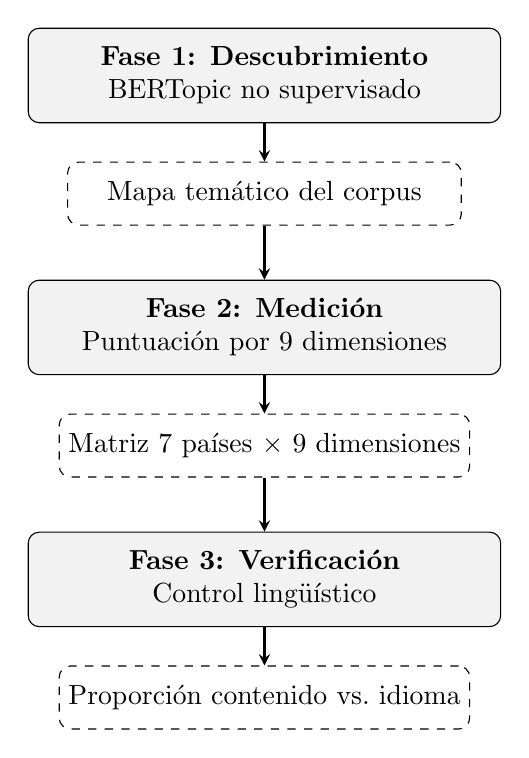
\begin{tikzpicture}[
    fase/.style={draw, rounded corners, minimum width=6cm, minimum height=1.2cm, align=center, fill=gray!10},
    resultado/.style={draw, dashed, rounded corners, minimum width=5cm, minimum height=0.8cm, align=center, fill=white},
    flecha/.style={->, thick, >=stealth}
]
\node[fase] (f1) at (0,0) {\textbf{Fase 1: Descubrimiento}\\BERTopic no supervisado};
\node[resultado] (r1) at (0,-1.5) {Mapa temático del corpus};

\node[fase] (f2) at (0,-3.2) {\textbf{Fase 2: Medición}\\Puntuación por 9 dimensiones};
\node[resultado] (r2) at (0,-4.7) {Matriz 7 países $\times$ 9 dimensiones};

\node[fase] (f3) at (0,-6.4) {\textbf{Fase 3: Verificación}\\Control lingüístico};
\node[resultado] (r3) at (0,-7.9) {Proporción contenido vs.\ idioma};

\draw[flecha] (f1) -- (r1);
\draw[flecha] (r1) -- (f2);
\draw[flecha] (f2) -- (r2);
\draw[flecha] (r2) -- (f3);
\draw[flecha] (f3) -- (r3);
\end{tikzpicture}
\caption{Secuencia analítica de tres fases. Elaboración propia.}
\label{fig:secuencia}
\end{figure}

La primera fase descubre los temas del corpus mediante el análisis no supervisado. Se alimentan todos los fragmentos al modelo de descubrimiento de temas, que los agrupa por afinidad semántica. Para evitar que los países con más texto dominen los resultados, se limita la muestra a un máximo de 80 fragmentos por país. Esta fase produce un mapa temático del corpus que no depende de las categorías del investigador.

La segunda fase mide cada documento contra las nueve dimensiones del marco analítico. Los párrafos ancla se comparan con los fragmentos de cada país y se calcula una puntuación de afinidad. El resultado es una matriz de siete países por nueve dimensiones que permite comparar qué temas enfatiza cada política.

La tercera fase verifica que las similitudes detectadas no sean un artefacto del idioma. El control lingüístico compara las similitudes entre países que comparten idioma (por ejemplo, Canadá y Australia, ambos en inglés) con las similitudes entre países de idiomas diferentes (por ejemplo, Canadá y Colombia). Si las similitudes entre países del mismo idioma son sistemáticamente más altas que las de idiomas distintos, esa diferencia mide el sesgo lingüístico del modelo. El control incluye también una línea base monolingüe: traducir todos los documentos al inglés y recalcular las similitudes permite aislar cuánta de la similitud original se debe al contenido y cuánta al idioma.

Para el caso de China, el análisis tiene dos niveles. En la comparación entre países, China está representada por un solo documento: la Guía de IA para educación básica de 2024 (K-12 se refiere al rango completo de educación preescolar a bachillerato en la nomenclatura anglosajona). En el análisis longitudinal, los siete documentos de China se comparan entre sí para observar cómo cambiaron las prioridades entre 2017 y 2025.


\section{Precedentes}

El uso de representaciones semánticas para analizar documentos de política pública no es nuevo. \citet{rodriguez2022embeddings} demostraron en el \textit{Journal of Politics} que los modelos de representación semántica capturan distinciones sustantivas relevantes para la ciencia política, y establecieron criterios para evaluar cuándo estos modelos funcionan bien y cuándo no. \citet{kozlowski2019geometry} usaron representaciones semánticas en el \textit{American Sociological Review} para analizar significados culturales, demostrando que estas herramientas capturan constructos sociales, no solo patrones superficiales de texto.

En el campo específico de las políticas de IA, \citet{fatima2020aipolicy} realizaron un análisis comparativo de planes nacionales de inteligencia artificial en 34 países, utilizando dimensiones analíticas similares a las de esta investigación. La librería NLP4Gov~\citep{nlp4gov2024} sistematizó herramientas de procesamiento de lenguaje natural para el análisis de políticas, incluyendo búsqueda semántica y comparación de documentos mediante representaciones similares a las que se emplean aquí.

Lo que esta investigación agrega respecto a estos precedentes es la combinación de tres elementos. El primero es el análisis no supervisado previo al marco analítico, que evita que las categorías del investigador determinen de antemano lo que el análisis encuentra. El segundo es la verificación del sesgo de idioma, que se incorporó porque los modelos multilingüe no separan perfectamente el contenido del idioma~\citep{conneau2020unsupervised}: sin esta verificación, dos documentos en inglés podrían obtener puntuaciones de similitud infladas simplemente por compartir idioma, no contenido. El tercero es el enfoque en políticas de educación en IA en lugar de estrategias nacionales de IA en general, lo que permite un análisis más específico de cómo los países abordan la dimensión educativa.
